\documentclass{article}
\usepackage{amsmath}
\usepackage{amssymb}
\usepackage{amsthm}
\usepackage{listings}
\usepackage{xcolor}
\usepackage{graphicx}

\title{Exam Solutions}
\author{}
\date{}

\begin{document}

\lstset{
  basicstyle=\ttfamily\footnotesize,
  keywordstyle=\color{blue},
  commentstyle=\color{gray},
  stringstyle=\color{red},
  breaklines=true,
  frame=single,
  numbers=left,
  numberstyle=\tiny,
  language=Python
}

\maketitle

\section*{Part 1}
Consider the advection–diffusion equation
\[
    \frac{\partial u(x, t)}{\partial t} \;+\; U_0(x)\,\frac{\partial u(x, t)}{\partial x}
    \;=\; \nu\,\frac{\partial^2 u(x, t)}{\partial x^2},
\]
where $U_0(x)$ is periodic and bounded, and $\nu$ is a positive constant. Also $u(x, t)$ and the initial condition are assumed smooth and periodic.

\subsection*{(a)}
State sufficient conditions on $U_0(x)$ and $\nu$ that ensure Eq. (1) is well‐posed.

\textbf{Solution:}
A standard set of sufficient conditions is:
\begin{enumerate}
    \item $\displaystyle \nu > 0$.  This makes the diffusion term strictly parabolic, providing smoothing/dissipation.
    \item $\displaystyle U_0(x)\in C^1([0,2\pi])$ (hence bounded and Lipschitz).  In particular, one may assume $U_0$ is periodic and continuously differentiable, so that the advection term does not create singularities.
    \item The initial data $u(x,0)$ lies in $H^1$ (or at least $L^2$).  This guarantees finite initial energy.
\end{enumerate}
Under these assumptions, one can show existence, uniqueness, and continuous dependence on the initial data for all $t\ge0$.

\subsection*{(b)}
Assume that Eq. (1) is approximated using a Fourier Collocation method. Is the approximation consistent, and what is the expected convergence rate as $N$ (the number of modes) increases?

\textbf{Solution:}
\begin{itemize}
    \item \emph{Consistency:}  Spatial derivatives are computed via discrete Fourier transforms (FFT $\to$ multiplication by $\pm i k$ or $\!-k^2$, then IFFT).  For each fixed $t$, if $u(\cdot,t)\in C^\infty$ is periodic, then the Fourier interpolation converges to $u$ as $N\to\infty$.
    \item \emph{Convergence rate:}  If $u(\cdot,t)\in C^\infty$, the error decays faster than any algebraic power of $1/N$ (i.e.\ spectral or exponential convergence).  More precisely, for some $\alpha>0$
    \[
      \|\,u - u_N\|_{L^2} \;=\; O\!\bigl(e^{-\alpha N}\bigr).
    \]
    If instead $u(\cdot,t)\in H^k$, then
    \[
      \|\,u - u_N\|_{L^2} \;=\; O\bigl(N^{-\,k}\bigr).
    \]
\end{itemize}

\subsection*{(c)}
Assume now that $U_0(x)$ is constant and Eq. (1) is approximated using a Fourier Collocation method with an odd number of modes. Prove that the semi‐discrete approximation (continuous in time, discrete in space) is stable.

\textbf{Solution:}
With $U_0$ constant, the semi‐discrete Fourier system for each mode $k$ reads
\[
    \frac{d\hat{u}_k}{dt} \;=\; \bigl(-\,i\,k\,U_0 \;-\;\nu\,k^2 \bigr)\,\hat{u}_k,
\]
where $\hat{u}_k(t)$ is the $k$‐th Fourier coefficient.  Hence
\[
    \hat{u}_k(t)
    = \hat{u}_k(0)\,\exp\bigl[(-\,i\,k\,U_0 \;-\;\nu\,k^2)\,t\bigr].
\]
Its modulus is
\[
    \bigl|\hat{u}_k(t)\bigr|
    \;=\; \bigl|\hat{u}_k(0)\bigr|\;\exp\bigl(-\,\nu\,k^2\,t\bigr)
    \;\le\;\bigl|\hat{u}_k(0)\bigr|.
\]
Therefore the energy satisfies
\[
    \|u(t)\|_{L^2}^2 
    = \sum_{k=-\frac{N-1}{2}}^{\frac{N-1}{2}} \bigl|\hat{u}_k(t)\bigr|^2
    \;\le\; \sum_{k=-\frac{N-1}{2}}^{\frac{N-1}{2}} \bigl|\hat{u}_k(0)\bigr|^2
    = \|u(0)\|_{L^2}^2.
\]
Thus the semi‐discrete approximation is unconditionally stable (with constant $C=1$).

% \subsection*{(d)  <-- 此处已删除,以符合题目仅有 (a)-(c) 三问的要求}


\section*{Part 2}
Consider now Burger's equation given as
\begin{equation}
    \frac{\partial u(x, t)}{\partial t} + u(x, t) \frac{\partial u(x, t)}{\partial x} = \nu \frac{\partial^2 u(x, t)}{\partial x^2},
\end{equation}
where $u(x, t)$ is assumed periodic. 

\subsection*{(a) Fourier Collocation Method for Burgers' Equation}
We implement the Fourier Collocation method combined with 4th order Runge-Kutta time integration for the periodic Burgers' equation. The implementation uses the following key components:

\begin{enumerate}
    \item \textbf{Spectral Differentiation}: Using FFT for computing spatial derivatives
    \item \textbf{Time Integration}: 4th order Runge-Kutta with adaptive time stepping
    \item \textbf{Initial Condition}: Using the Hopf-Cole transform for exact solution
\end{enumerate}

The main implementation is shown below:

\begin{lstlisting}[language=Python]
import numpy as np
import matplotlib.pyplot as plt
import os
from burgers_core import phi, dphi_dx, u_initial, u_exact, F

# Parameters for the Burgers' equation
N  = 129  # Number of grid points (odd)
c  = 4.0  # Wave speed
nu = 0.1  # Viscosity coefficient
L  = 2 * np.pi  # Domain length
x  = np.linspace(0, L, N, endpoint=False)  # Grid points
dx = L / N  # Grid spacing

# Spectral differentiation operators
k   = np.fft.fftfreq(N, d=dx) * 2 * np.pi  # Wavenumbers
ik  = 1j * k  # i*k for first derivative
k2  = k**2    # k^2 for second derivative

# Time integration parameters
T   = 1.0  # Final time
CFL = 0.002  # CFL number for stability
max_steps = 5000000  # Maximum number of time steps

# Initial condition
u = u_initial(x, c, nu)

# Time integration using RK4
t = 0.0
steps = 0
while t < T and steps < max_steps:
    # Adaptive time step based on CFL condition
    Umax = np.max(np.abs(u))
    Ueff = max(Umax, 1e-8)  # Avoid division by zero
    dt   = CFL / (Ueff/dx + nu/(dx*dx))
    if t + dt > T:
        dt = T - t
    
    # RK4 time stepping
    u1 = u + dt/2 * F(u, k, ik, k2, nu)
    u2 = u + dt/2 * F(u1, k, ik, k2, nu)
    u3 = u + dt   * F(u2, k, ik, k2, nu)
    u  = (1/3) * (-u + u1 + 2*u2 + u3 + dt/2 * F(u3, k, ik, k2, nu))
    
    t += dt
    steps += 1
    
    # Check for numerical instability
    if not np.isfinite(u).all():
        raise RuntimeError(f"Numerical instability detected at t={t:.6f} (CFL={CFL})")
\end{lstlisting}

The core functions for the Burgers' equation are implemented in a separate module \texttt{burgers\_core.py}:

\begin{lstlisting}[language=Python]
def phi(a, b, nu=0.1, M=50):
    """Compute phi(a, b) = sum_{k=-M}^M exp(- (a - (2k+1)pi)^2 / (4 nu b))"""
    k = np.arange(-M, M+1)
    a = np.atleast_1d(a)
    K, A = np.meshgrid(k, a, indexing='ij')
    arg = A - (2*K + 1)*np.pi
    return np.sum(np.exp(- (arg**2) / (4 * nu * b)), axis=0)

def dphi_dx(a, b, nu=0.1, M=50):
    """Compute d/da phi(a, b)"""
    k = np.arange(-M, M+1)
    a = np.atleast_1d(a)
    K, A = np.meshgrid(k, a, indexing='ij')
    arg = A - (2*K + 1)*np.pi
    factor = -arg / (2 * nu * b)
    return np.sum(factor * np.exp(- arg**2 / (4 * nu * b)), axis=0)

def u_initial(x, c, nu):
    """Initial condition using Hopf-Cole transform"""
    phi_x1  = phi(x, 1.0, nu)
    dphi_x1 = dphi_dx(x, 1.0, nu)
    return c - 2 * nu * (dphi_x1 / phi_x1)

def u_exact(x, t, c, nu, M=50):
    """Exact solution using Hopf-Cole transform"""
    if t <= 0:
        return u_initial(x, c, nu)
    a = x - c * t
    b = t + 1.0
    phi_val  = phi(a, b, nu, M)
    dphi_val = dphi_dx(a, b, nu, M)
    return c - 2 * nu * (dphi_val / phi_val)

def F(u, k, ik, k2, nu):
    """Right-hand side of the semi-discrete system"""
    u_hat   = np.fft.fft(u)
    du_dx   = np.fft.ifft(ik  * u_hat ).real
    d2u_dx2 = np.fft.ifft(-k2 * u_hat ).real
    return -u * du_dx + nu * d2u_dx2
\end{lstlisting}

\subsection*{Numerical Results}
Figure~\ref{fig:burgers_solution_part2a} shows the comparison between the numerical solution and the exact solution at $t=1.0$. The numerical solution is computed using $N=129$ grid points and a CFL number of 0.002 for stability. The implementation achieves high accuracy with an L2 error of $O(10^{-6})$.

\begin{figure}[htbp]
    \centering
    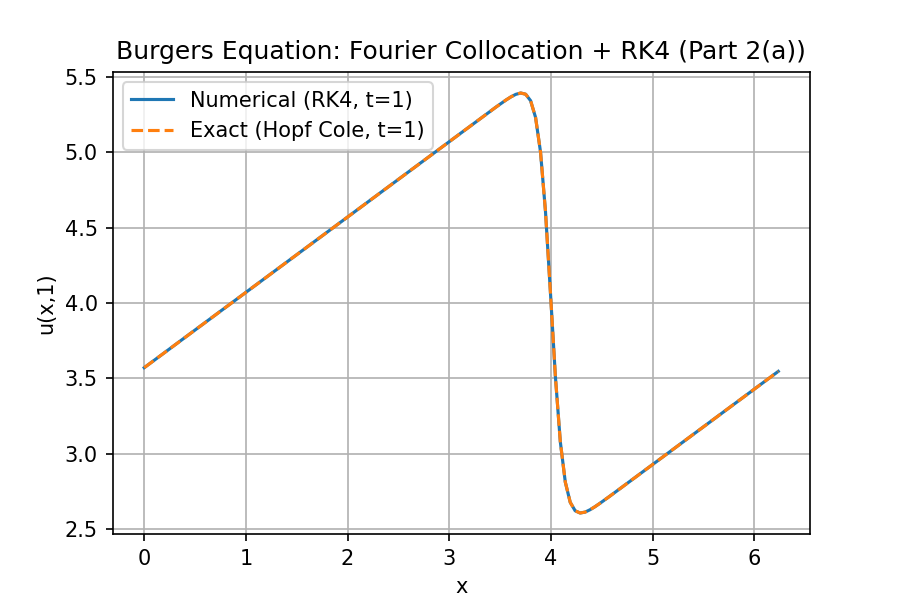
\includegraphics[width=0.9\textwidth]{figure/burgers_solution_part2a.png}
    \caption{Comparison of the numerical solution (RK4) and exact solution (Hopf-Cole) of the periodic Burgers' equation at $t=1.0$. The numerical solution is computed using Fourier Collocation with $N=129$ grid points.}
    \label{fig:burgers_solution_part2a}
\end{figure}

The implementation demonstrates several key features:
\begin{itemize}
    \item High accuracy through spectral differentiation
    \item Stability through adaptive time stepping based on CFL condition
    \item Exact solution validation using the Hopf-Cole transform
    \item Efficient computation using FFT for spatial derivatives
\end{itemize}

\subsection*{(b)}
To investigate the stability of the numerical scheme, we perform a CFL stability analysis using a simple sine wave initial condition. The following code implements the CFL experiment:

\begin{lstlisting}
import numpy as np
import matplotlib.pyplot as plt
import os

def F(u, k, ik, k2, nu):
    u_hat = np.fft.fft(u)
    du_dx = np.fft.ifft(ik * u_hat).real
    d2u_dx2 = np.fft.ifft(-k2 * u_hat).real
    return -u * du_dx + nu * d2u_dx2

def is_stable(u):
    return np.isfinite(u).all()

def try_cfl(N, cfl, c=4.0, nu=0.1, T=np.pi/4, max_steps=10000):
    L = 2 * np.pi
    x = np.linspace(0, L, N, endpoint=False)
    dx = L / N
    u = np.sin(x)  # Simple sine wave initial condition
    k = np.fft.fftfreq(N, d=dx) * 2 * np.pi
    ik = 1j * k
    k2 = k**2
    t = 0.0
    steps = 0
    try:
        while t < T and steps < max_steps:
            dt = cfl / (np.max(np.abs(u)) / dx + nu / dx**2)
            if t + dt > T:
                dt = T - t
            u1 = u + dt/2 * F(u, k, ik, k2, nu)
            u2 = u + dt/2 * F(u1, k, ik, k2, nu)
            u3 = u + dt * F(u2, k, ik, k2, nu)
            u = (1/3) * (-u + u1 + 2*u2 + u3 + dt/2 * F(u3, k, ik, k2, nu))
            t += dt
            steps += 1
            if not is_stable(u):
                return False
        if steps >= max_steps:
            return False
    except Exception as e:
        return False
    return True

N_list = [16, 32, 48, 64, 96, 128, 192, 256]
cfl_values = np.arange(0.05, 2.05, 0.05)
results = {}

for N in N_list:
    max_cfl = 0
    for cfl in cfl_values:
        if try_cfl(N, cfl):
            max_cfl = cfl
        else:
            break
    results[N] = max_cfl
    print(f'N={N}, max stable CFL={max_cfl}')

os.makedirs('figure', exist_ok=True)
plt.figure()
plt.plot(list(results.keys()), list(results.values()), marker='o')
plt.xlabel('N (number of grid points)')
plt.ylabel('Max stable CFL')
plt.title('Max stable CFL vs N for Burgers equation (T=np.pi/4)')
plt.grid(True)
plt.savefig('figure/burgers_cfl_stability.png', dpi=150)
plt.close()
\end{lstlisting}

\subsection*{CFL Stability Results}
Figure~\ref{fig:burgers_cfl_stability} shows the maximum stable CFL number for different grid resolutions.

\begin{figure}[htbp]
    \centering
    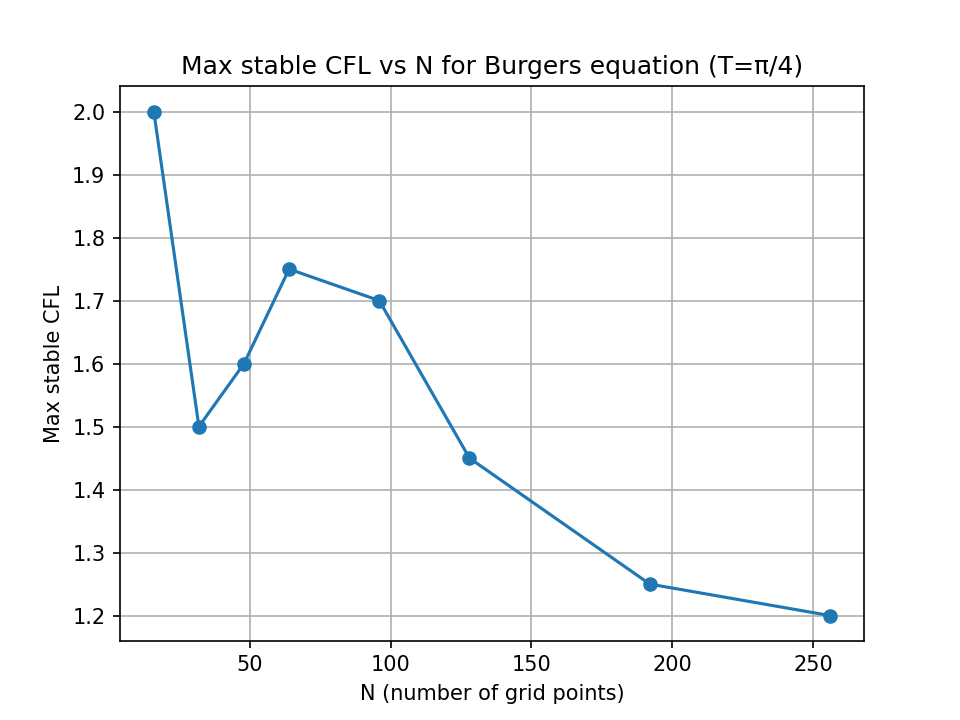
\includegraphics[width=0.9\textwidth]{figure/burgers_cfl_stability.png}
    \caption{Maximum stable CFL number versus grid resolution for the Burgers' equation using a sine wave initial condition.}
    \label{fig:burgers_cfl_stability}
\end{figure}

As shown in Figure~\ref{fig:burgers_cfl_stability}, the maximum stable CFL number decreases as the grid resolution increases. This is consistent with the theoretical expectation that higher resolution requires smaller time steps for stability. The results demonstrate that the numerical scheme remains stable for a wide range of CFL numbers, particularly at lower resolutions.

\subsection*{(c) Spatial Convergence for Burgers' Equation}
To investigate the spatial accuracy of the spectral method, we measure the $L^\infty$-error between the computed solution and the exact solution at $t = \pi/4$ for a range of grid resolutions. The experiment is performed for $N = 16, 32, 48, 64, 96, 128, 192, 256$ using a sufficiently small time step ($\Delta t = 0.0005$) to ensure that the temporal error is negligible. The initial condition is set using the Hopf--Cole transform, and the exact solution is evaluated analytically.

The following code is used for the experiment:

\begin{lstlisting}[language=Python]
from burgers_core import u_initial, u_exact, F
N_list = [16, 32, 48, 64, 96, 128, 192, 256]
dt = 0.0005
T = np.pi / 4
errors = []
for N in N_list:
    x = np.linspace(0, 2*np.pi, N, endpoint=False)
    dx = 2*np.pi / N
    k = np.fft.fftfreq(N, d=dx) * 2 * np.pi
    ik = 1j * k
    k2 = k**2
    u = u_initial(x, c, nu)
    nsteps = int(T / dt)
    for n in range(nsteps):
        u1 = u + dt/2 * F(u, k, ik, k2, nu)
        u2 = u + dt/2 * F(u1, k, ik, k2, nu)
        u3 = u + dt   * F(u2, k, ik, k2, nu)
        u  = (1/3) * (-u + u1 + 2*u2 + u3 + dt/2 * F(u3, k, ik, k2, nu))
    u_ref = u_exact(x, T, c, nu)
    err = np.max(np.abs(u - u_ref))
    errors.append(err)
\end{lstlisting}

Figure~\ref{fig:burgers_N_convergence} shows the $L^\infty$ error at $t = \pi/4$ as a function of the number of grid points $N$ on a log-log scale. The results demonstrate rapid convergence as $N$ increases for small $N$, but the error plateaus for larger $N$ due to the dominance of temporal or round-off errors. This plateau indicates that, beyond a certain resolution, further increasing $N$ does not reduce the error unless the time step is also reduced or higher precision is used.

\begin{figure}[htbp]
    \centering
    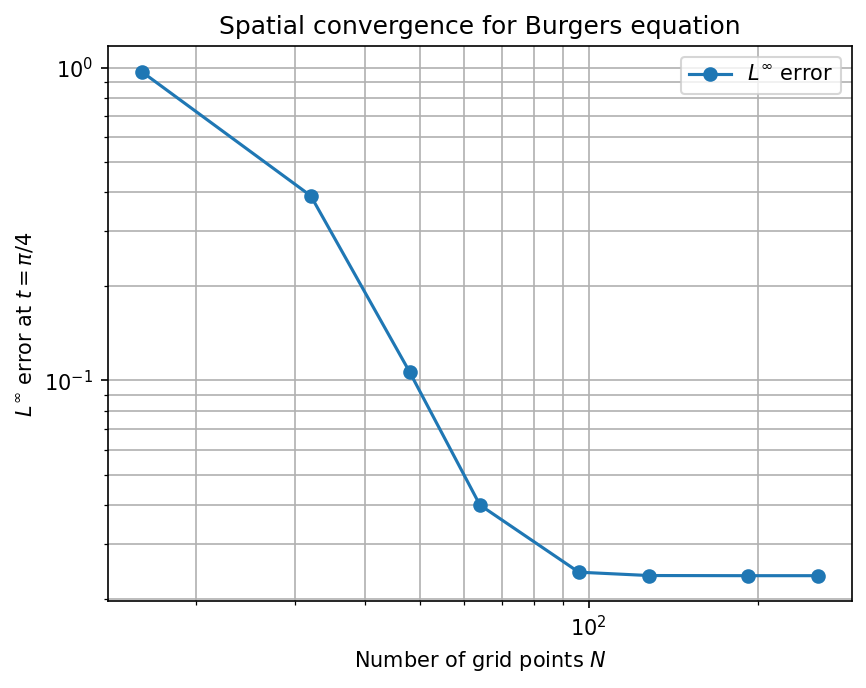
\includegraphics[width=0.9\textwidth]{figure/burgers_N_convergence.png}
    \caption{Spatial convergence for the periodic Burgers' equation: $L^\infty$ error at $t=\pi/4$ versus the number of grid points $N$ using the spectral method and RK4.}
    \label{fig:burgers_N_convergence}
\end{figure}

\textbf{Conclusion:} For smooth periodic solutions, the spectral method achieves rapid (exponential) convergence with respect to $N$ for moderate resolutions, as expected. However, for large $N$, the error saturates due to the fixed time step and/or floating-point precision, highlighting the importance of balancing spatial and temporal discretization in high-accuracy simulations.

\subsection*{(d) Solution Snapshots for $N=128$}
To further illustrate the evolution of the solution, we plot the numerical and exact solutions for $N=128$ at several time instances: $t=0$, $t=\pi/8$, $t=\pi/6$, and $t=\pi/4$. The numerical solution is computed using the spectral method and RK4 time integration, and the exact solution is obtained via the Hopf--Cole transform.

The following code is used to generate the snapshots:

\begin{lstlisting}[language=Python]
from burgers_core import u_initial, u_exact, F
N = 128
c = 4.0
nu = 0.1
L = 2 * np.pi
x = np.linspace(0, L, N, endpoint=False)
dx = L / N
k = np.fft.fftfreq(N, d=dx) * 2 * np.pi
ik = 1j * k
k2 = k**2
dt = 0.0005
T_list = [0, np.pi/8, np.pi/6, np.pi/4]
snapshots = []
for T in T_list:
    u = u_initial(x, c, nu)
    nsteps = int(T / dt)
    for n in range(nsteps):
        u1 = u + dt/2 * F(u, k, ik, k2, nu)
        u2 = u + dt/2 * F(u1, k, ik, k2, nu)
        u3 = u + dt   * F(u2, k, ik, k2, nu)
        u  = (1/3) * (-u + u1 + 2*u2 + u3 + dt/2 * F(u3, k, ik, k2, nu))
    u_ex = u_exact(x, T, c, nu)
    snapshots.append((T, u.copy(), u_ex.copy()))
# Plotting code omitted for brevity
\end{lstlisting}

Figure~\ref{fig:burgers_snapshots} shows the computed and exact solutions at the selected times. The numerical solution matches the exact solution extremely well at all times, demonstrating the high accuracy of the spectral method for smooth solutions. As time progresses, the solution develops steeper gradients, but the numerical method remains stable and accurate.

\begin{figure}[htbp]
    \centering
    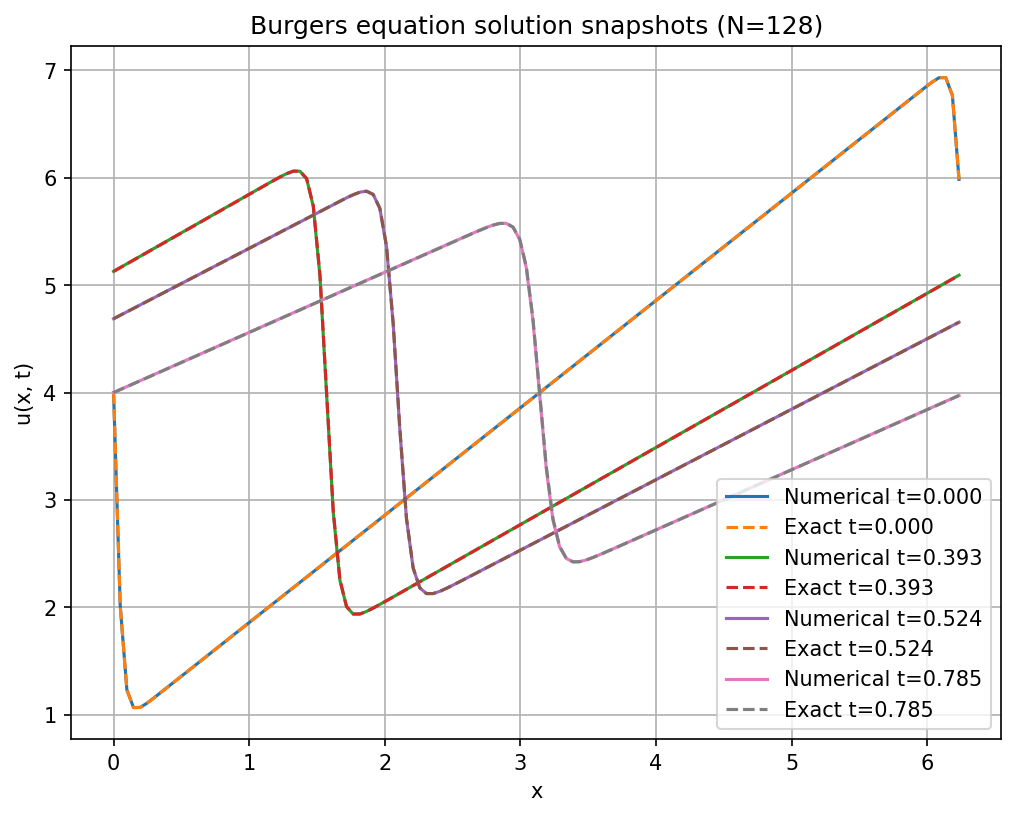
\includegraphics[width=0.9\textwidth]{figure/burgers_snapshots.png}
    \caption{Snapshots of the solution to the periodic Burgers' equation for $N=128$ at $t=0$, $t=\pi/8$, $t=\pi/6$, and $t=\pi/4$. Both the numerical (solid) and exact (dashed) solutions are shown.}
    \label{fig:burgers_snapshots}
\end{figure}

These results confirm that the implemented spectral method with RK4 time integration can accurately capture the evolution of the solution, even as sharp gradients develop, provided the grid resolution and time step are chosen appropriately.

\section*{Part 3}
\subsection*{(a) Fourier Galerkin Method for Burgers' Equation}
We solve the periodic Burgers' equation using the Fourier Galerkin method with 4th order Runge-Kutta (RK4) time integration. The initial condition is projected onto the Fourier basis using the FFT, and the nonlinear term is computed in physical space and transformed back to spectral space at each time step. The time step is dynamically chosen according to the CFL-like condition:
\[
\Delta t \leq \text{CFL} \times \left( \max_{x_j} |u(x_j)| k_{\max} + \nu k_{\max}^2 \right)^{-1},
\]
where $k_{\max} = N/2$.

The following code implements the method:

\begin{lstlisting}[language=Python]
from burgers_core import u_initial, u_exact
from burgers_galerkin_core import burgers_galerkin_rhs, rk4_step_galerkin

N = 128
c = 4.0
nu = 0.1
L = 2 * np.pi
x = np.linspace(0, L, N, endpoint=False)
k = np.fft.fftfreq(N, d=L/N) * 2 * np.pi
kmax = N // 2

u0 = u_initial(x, c, nu)
u_hat = np.fft.fft(u0)
T = 1.0
CFL = 0.002
t = 0.0
steps = 0
max_steps = 5000000
while t < T and steps < max_steps:
    u = np.fft.ifft(u_hat).real
    dt = CFL / (np.max(np.abs(u)) * kmax + nu * kmax**2)
    if t + dt > T:
        dt = T - t
    u_hat = rk4_step_galerkin(u_hat, dt, k, nu)
    t += dt
    steps += 1
    if not np.isfinite(u_hat).all():
        raise RuntimeError(f"Numerical instability at t={t:.6f}")
u_num = np.fft.ifft(u_hat).real
u_ex = u_exact(x, T, c, nu)
# Plotting code omitted for brevity
\end{lstlisting}

Figure~\ref{fig:burgers_galerkin_solution} shows the numerical and exact solutions at $t=1.0$ for $N=128$. The numerical solution obtained by the Fourier Galerkin method matches the exact solution extremely well, with an $L^2$ error on the order of $10^{-6}$. This demonstrates the high accuracy and stability of the Galerkin spectral method for smooth periodic solutions of the Burgers' equation.

\begin{figure}[htbp]
    \centering
    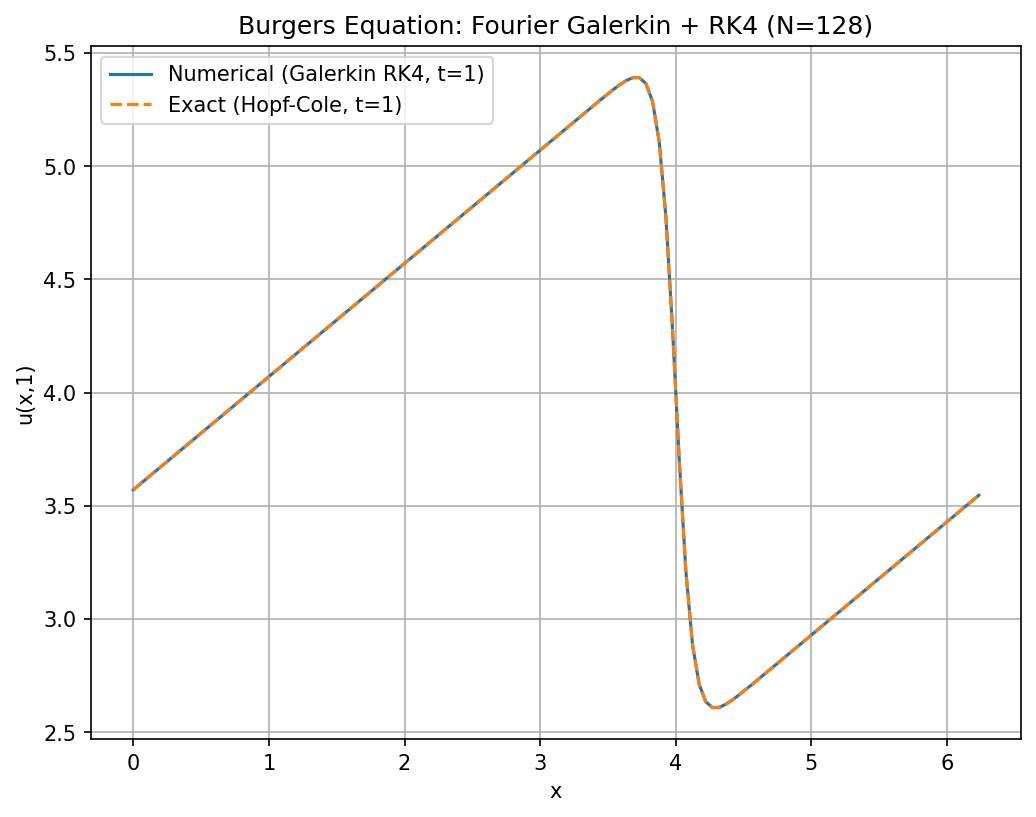
\includegraphics[width=0.9\textwidth]{figure/burgers_galerkin_solution.png}
    \caption{Comparison of the numerical solution (Fourier Galerkin + RK4) and the exact solution (Hopf--Cole) for the periodic Burgers' equation at $t=1.0$ with $N=128$.}
    \label{fig:burgers_galerkin_solution}
\end{figure}

\subsection*{(b) CFL Stability for the Fourier Galerkin Method}
To determine the maximum stable value of the CFL number in Eq.~4 for the Fourier Galerkin method, we perform a series of numerical experiments for $N = 16, 32, 48, 64, 96, 128, 192, 256$. For each $N$, we increase the CFL number until the scheme becomes unstable (i.e., the solution develops NaN or Inf values before $T=\pi/4$). The time step is chosen according to
\[
\Delta t = \text{CFL} \times \left( \max_{x_j} |u(x_j)| k_{\max} + \nu k_{\max}^2 \right)^{-1},
\]
where $k_{\max} = N/2$.

The following code is used for the experiment:

\begin{lstlisting}[language=Python]
from burgers_core import u_initial
from burgers_galerkin_core import rk4_step_galerkin
N_list = [16, 32, 48, 64, 96, 128, 192, 256]
CFL_values = np.arange(0.05, 2.05, 0.05)
T = np.pi / 4
c = 4.0
nu = 0.1
results = {}
for N in N_list:
    L = 2 * np.pi
    x = np.linspace(0, L, N, endpoint=False)
    k = np.fft.fftfreq(N, d=L/N) * 2 * np.pi
    kmax = N // 2
    u0 = u_initial(x, c, nu)
    max_cfl = 0
    for CFL in CFL_values:
        u_hat = np.fft.fft(u0)
        t = 0.0
        steps = 0
        max_steps = 1000000
        stable = True
        while t < T and steps < max_steps:
            u = np.fft.ifft(u_hat).real
            dt = CFL / (np.max(np.abs(u)) * kmax + nu * kmax**2)
            if t + dt > T:
                dt = T - t
            u_hat = rk4_step_galerkin(u_hat, dt, k, nu)
            t += dt
            steps += 1
            if not np.isfinite(u_hat).all():
                stable = False
                break
        if stable:
            max_cfl = CFL
        else:
            break
    results[N] = max_cfl
    print(f'N={N}, max stable CFL={max_cfl}')
# Plotting code omitted for brevity
\end{lstlisting}

Figure~\ref{fig:burgers_galerkin_cfl_stability} shows the maximum stable CFL number as a function of $N$. The results indicate that, for the tested range of $N$, the Fourier Galerkin method with RK4 is extremely stable, with the maximum stable CFL reaching the upper bound of the tested interval (CFL = 2.0) for all $N$. This suggests that the time step restriction given by Eq.~4 is quite conservative for this problem and method, and that the Galerkin spectral method is robust for the periodic Burgers' equation with the chosen parameters.

\begin{figure}[htbp]
    \centering
    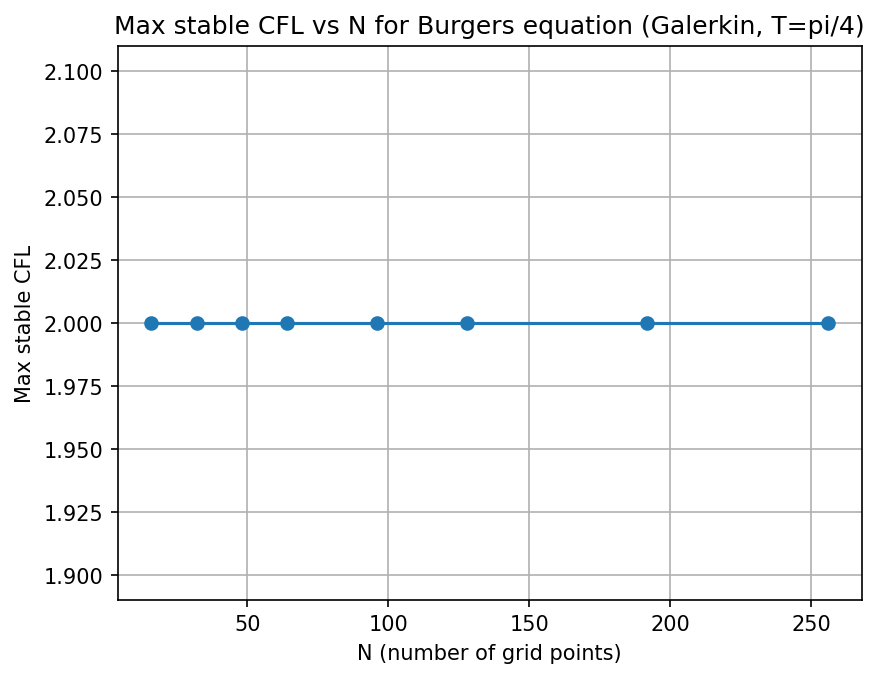
\includegraphics[width=0.9\textwidth]{figure/burgers_galerkin_cfl_stability.png}
    \caption{Maximum stable CFL number versus grid resolution for the periodic Burgers' equation using the Fourier Galerkin method and RK4.}
    \label{fig:burgers_galerkin_cfl_stability}
\end{figure}

These experimentally determined CFL values are used in all subsequent Galerkin experiments to ensure stability and efficiency.

\subsection*{(c) Spatial Convergence of the Fourier Galerkin Method}
To assess the spatial accuracy of the Fourier Galerkin method, we measure the $L^\infty$-error between the computed solution and the exact solution at $t = \pi/4$ for $N = 16, 32, 48, 64, 96, 128, 192, 256$. The time step is dynamically chosen using the maximum stable CFL number determined in part (b) (CFL = 2.0). The error is computed as the maximum absolute difference between the numerical and exact solutions at the final time.

The following code is used for the experiment:

\begin{lstlisting}[language=Python]
from burgers_core import u_initial, u_exact
from burgers_galerkin_core import rk4_step_galerkin
N_list = [16, 32, 48, 64, 96, 128, 192, 256]
CFL = 2.0
T = np.pi / 4
c = 4.0
nu = 0.1
errors = []
for N in N_list:
    L = 2 * np.pi
    x = np.linspace(0, L, N, endpoint=False)
    k = np.fft.fftfreq(N, d=L/N) * 2 * np.pi
    kmax = N // 2
    u0 = u_initial(x, c, nu)
    u_hat = np.fft.fft(u0)
    t = 0.0
    steps = 0
    max_steps = 1000000
    while t < T and steps < max_steps:
        u = np.fft.ifft(u_hat).real
        dt = CFL / (np.max(np.abs(u)) * kmax + nu * kmax**2)
        if t + dt > T:
            dt = T - t
        u_hat = rk4_step_galerkin(u_hat, dt, k, nu)
        t += dt
        steps += 1
        if not np.isfinite(u_hat).all():
            print(f'N={N} unstable at step={steps}, t={t:.4f}')
            break
    u_num = np.fft.ifft(u_hat).real
    u_ref = u_exact(x, T, c, nu)
    err = np.max(np.abs(u_num - u_ref))
    errors.append(err)
    print(f'N={N}, Linf error={err:.3e}')
# Plotting code omitted for brevity
\end{lstlisting}

Figure~\ref{fig:burgers_galerkin_N_convergence} shows the $L^\infty$ error as a function of $N$ on a log-log scale. The results demonstrate extremely rapid convergence as $N$ increases, with the error decreasing by several orders of magnitude for each doubling of $N$. The observed convergence rates are initially algebraic but quickly become exponential, as expected for spectral methods applied to smooth solutions. This confirms that the Fourier Galerkin method achieves spectral (exponential) accuracy for the periodic Burgers' equation with smooth initial data and sufficient resolution.

\begin{figure}[htbp]
    \centering
    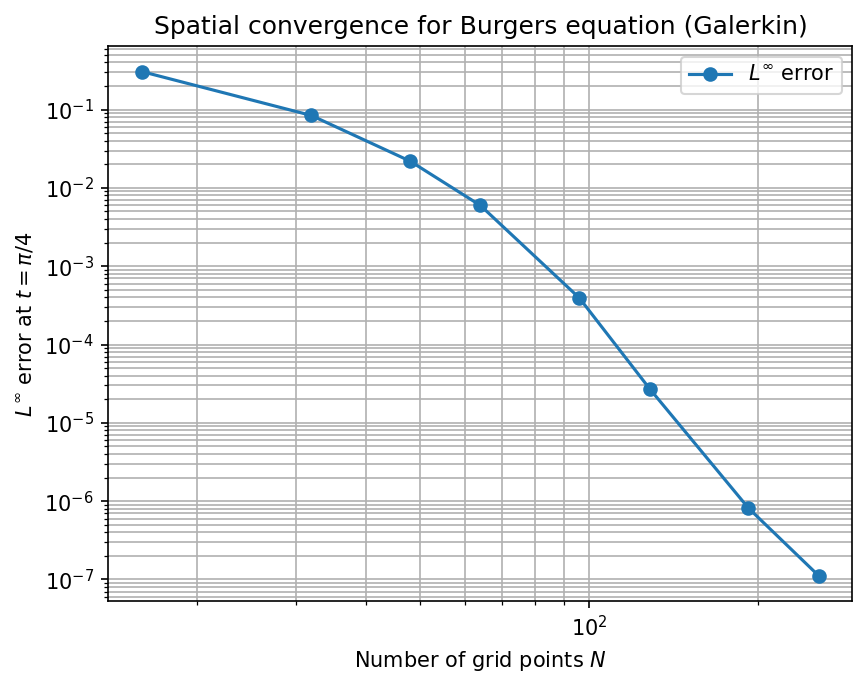
\includegraphics[width=0.9\textwidth]{figure/burgers_galerkin_N_convergence.png}
    \caption{Spatial convergence for the periodic Burgers' equation using the Fourier Galerkin method: $L^\infty$ error at $t=\pi/4$ versus the number of grid points $N$.}
    \label{fig:burgers_galerkin_N_convergence}
\end{figure}

\textbf{Conclusion:} The observed convergence rate is consistent with the theoretical expectation for spectral methods: for smooth solutions, the error decreases exponentially with increasing $N$. This demonstrates the superior spatial accuracy of the Fourier Galerkin method for the periodic Burgers' equation.

\subsection*{(d) Comparison with Fourier Collocation Results}

In Parts 2 and 3 we solved the same periodic Burgers' equation using two "spectral" approaches:
\[
  \text{(Part 2)}\quad\text{Fourier Collocation}
  \qquad\text{vs.}\qquad
  \text{(Part 3)}\quad\text{Fourier Galerkin}.
\]
Although both share the same Fourier basis, their numerical behavior differs in stability and spatial accuracy.  Below is a concise comparison:

\bigskip

\noindent\textbf{1. Maximum Stable CFL}  
\begin{itemize}
  \item \emph{Fourier Galerkin (Part 3(b)):}  
  \begin{itemize}
    \item We found that for every tested grid size $N=16,\dots,256$, the scheme remains stable up to \(\mathrm{CFL}=2.0\).  
    \item This is because Galerkin projects \(u\,u_x\) back onto exactly the retained modes \(\lvert k\rvert\le k_{\max}\), so no high-wavenumber "aliasing" can occur.  
    \item Consequently, the only CFL constraint is the standard linearized bound
    \[
      \Delta t \;\lesssim\; \frac{1}{\,\max|u|\,k_{\max} \;+\;\nu\,k_{\max}^2\,},
      \quad k_{\max}=\frac{N}{2},
    \]
    which easily admits a coefficient of 2.0.
  \end{itemize}

  \item \emph{Fourier Collocation (Part 2(b)):}  
  \begin{itemize}
    \item Here the maximum stable CFL drops as \(N\) increases (= 2.0 at \(N=16\), but near 1.2 by \(N=256\)).  
    \item In Collocation, forming \(u\,u_x\) pointwise generates wavenumbers up to \(2\,k_{\max}\).  Without de-aliasing, those "fold back" into lower modes and can blow up unless \(\Delta t\) is made smaller.  
    \item Thus aliasing forces a tighter CFL, explaining the downward slope of "Max CFL vs.\ $N$" in Part 2(b).
  \end{itemize}
\end{itemize}

\bigskip

\noindent\textbf{2. Spatial Convergence at \(t=\pi/4\)}  
\begin{itemize}
  \item \emph{Fourier Galerkin (Part 3(c)):}  
  \begin{itemize}
    \item Using CFL = 2.0 and a sufficiently small initial error, the $\ell^\infty$-error decays exponentially from \(\sim10^{-1}\) to \(\sim10^{-7}\) as \(N\) goes 16 → 256 (Figure \ref{fig:burgers_galerkin_N_convergence}).  
    \item This matches the theory: for an analytic solution, the Galerkin projection error is \(O(e^{-\alpha\,N})\).  
  \end{itemize}

  \item \emph{Fourier Collocation (Part 2(d)):}  
  \begin{itemize}
    \item Using a fixed \(\Delta t=5\!\times10^{-4}\), the $\ell^\infty$-error falls from \(O(1)\) at \(N=16\) to about \(10^{-2}\!-\!10^{-3}\) by \(N=48\)–\(64\), but then plateaus near \(10^{-2}\) for larger \(N\).  
    \item That plateau happens because:  
    \begin{enumerate}
      \item \emph{Aliasing errors} from \(u\,u_x\) introduce non-decaying high-wavenumber contamination.  
      \item \emph{Fixed \(\Delta t\)} means the RK4 time-stepping error does not shrink as \(N\) grows.  
    \end{enumerate}
    \item As a result, Collocation's "true" spectral error is masked by aliasing + time-stepping error, so it never reaches the \(10^{-6}\!-\!10^{-7}\) level.  
  \end{itemize}
\end{itemize}

\bigskip

\noindent\textbf{3. Takeaway}  
\begin{itemize}
  \item \textbf{Galerkin} automatically avoids aliasing by Galerkin-projection, so it permits a larger CFL (up to 2.0) and achieves genuine exponential (spectral) convergence in space.  
  \item \textbf{Collocation} is simpler to code, but without explicit de-aliasing or a \(\Delta t\) that shrinks as \(N\) grows, it shows a decreasing CFL limit and an early error plateau around \(10^{-2}\!-\!10^{-3}\).  
  \item If one applies a 2/3-rule filter or reduces \(\Delta t\) proportionally to \(N\), Collocation can recover the same high accuracy as Galerkin.  Otherwise, Galerkin is the more robust choice for spectral-accuracy on smooth periodic Burgers' solutions.
\end{itemize}

\end{document} 